\documentclass[letterpaper]{article} % DO NOT CHANGE THIS
\usepackage[submission]{aaai2027}  % DO NOT CHANGE THIS
% The serif, sans-serif, and monospaced fonts are loaded automatically by
% aaai2027.sty (newtxtext, helvet, courier). DO NOT add \usepackage{times},
% \usepackage{helvet}, \usepackage{courier}, or any other font package.
\usepackage[hyphens]{url}  % DO NOT CHANGE THIS
\usepackage{graphicx} % DO NOT CHANGE THIS
\urlstyle{rm} % DO NOT CHANGE THIS
\def\UrlFont{\rm}  % DO NOT CHANGE THIS
\usepackage{natbib}  % DO NOT CHANGE THIS AND DO NOT ADD ANY OPTIONS TO IT
\usepackage{caption} % DO NOT CHANGE THIS AND DO NOT ADD ANY OPTIONS TO IT
\frenchspacing  % DO NOT CHANGE THIS
%
% These are recommended to typeset algorithms but not required. See the subsubsection on algorithms. Remove them if you don't have algorithms in your paper.
\usepackage{algorithm}
\usepackage{algorithmic}
\usepackage{amsmath}
\usepackage{multirow}
%
% These are recommended to typeset listings but not required. See the subsubsection on listing. Remove this block if you don't have listings in your paper.
\usepackage{newfloat}
\usepackage{listings}
\DeclareCaptionStyle{ruled}{labelfont=normalfont,labelsep=colon,strut=off} % DO NOT CHANGE THIS
\lstset{%
	basicstyle={\footnotesize\ttfamily},% footnotesize acceptable for monospace
	numbers=left,numberstyle=\footnotesize,xleftmargin=2em,% show line numbers, remove this entire line if you don't want the numbers.
	aboveskip=0pt,belowskip=0pt,%
	showstringspaces=false,tabsize=2,breaklines=true}
\floatstyle{ruled}
\newfloat{listing}{tb}{lst}{}
\floatname{listing}{Listing}

%
% Recommended for better-looking tables
\usepackage{booktabs}
\usepackage{pifont}

%
% Keep the \pdfinfo as shown here. There's no need
% for you to add the /Title and /Author tags.
\pdfinfo{
/TemplateVersion (2027.1)
}

% DISALLOWED PACKAGES
% \usepackage{authblk} -- This package is specifically forbidden
% \usepackage{balance} -- This package is specifically forbidden
% \usepackage{CJK} -- This package is specifically forbidden
% \usepackage{float} -- This package is specifically forbidden
% \usepackage{flushend} -- This package is specifically forbidden
% \usepackage{fullpage} -- This package is specifically forbidden
% \usepackage{geometry} -- This package is specifically forbidden
% \usepackage{hyperref} -- This package is specifically forbidden
% \usepackage{navigator} -- This package is specifically forbidden
% (or any other package that embeds links such as navigator or hyperref)
% \usepackage{indentfirst} -- This package is specifically forbidden
% \usepackage{layout} -- This package is specifically forbidden
% \usepackage{multicol} -- This package is specifically forbidden
% \usepackage{nameref} -- This package is specifically forbidden
% \usepackage{savetrees} -- This package is specifically forbidden
% \usepackage{setspace} -- This package is specifically forbidden
% \usepackage{stfloats} -- This package is specifically forbidden
% \usepackage{tabu} -- This package is specifically forbidden
% \usepackage{titlesec} -- This package is specifically forbidden
% \usepackage{tocbibind} -- This package is specifically forbidden
% \usepackage{ulem} -- This package is specifically forbidden
% \usepackage{wrapfig} -- This package is specifically forbidden
% DISALLOWED COMMANDS
% \nocopyright -- Your paper will not be published if you use this command
% \addtolength -- This command may not be used
% \balance -- This command may not be used
% \baselinestretch -- Your paper will not be published if you use this command
% \clearpage -- No page breaks of any kind may be used for the final version of your paper
% \columnsep -- This command may not be used
% \newpage -- No page breaks of any kind may be used for the final version of your paper
% \pagebreak -- No page breaks of any kind may be used for the final version of your paper
% \pagestyle -- This command may not be used
% \tiny -- This is not an acceptable font size.
% \vspace{- -- No negative value may be used in proximity of a caption, figure, table, section, subsection, subsubsection, or reference
% \vskip{- -- No negative value may be used to alter spacing above or below a caption, figure, table, section, subsection, subsubsection, or reference

\setcounter{secnumdepth}{0} %May be changed to 1 or 2 if section numbers are desired.

% The file aaai2027.sty is the style file for AAAI Press
% proceedings, working notes, and technical reports.
%

% Title

% Your title must be in mixed case, not sentence case.
% That means all verbs (including short verbs like be, is, using,and go),
% nouns, adverbs, adjectives should be capitalized, including both words in hyphenated terms, while
% articles, conjunctions, and prepositions are lower case unless they
% directly follow a colon or long dash
\newcommand{\methodname}{TextComp} 
\title{TextComp: Text-Guided Learning for Compressed Video Action Recognition} % Replace with your title

\author{
    %Authors
    % All authors must be in the same font size and format.
    Written by AAAI Press Staff\textsuperscript{\rm 1}\thanks{With help from the AAAI Publications Committee.}\\
    AAAI Style Contributions by Peter Patel Schneider,
    Sunil Issar,\\
    J. Scott Penberthy,
    George Ferguson,
    Hans Guesgen,
    Francisco Cruz\equalcontrib\corresponding,
    Marc Pujol-Gonzalez\equalcontrib\corresponding
}
\affiliations{
    %Afiliations
    \textsuperscript{\rm 1}Association for the Advancement of Artificial Intelligence\\
    % If you have multiple authors and multiple affiliations
    % use superscripts in text and roman font to identify them.
    % For example,

    % Sunil Issar\textsuperscript{\rm 2},
    % J. Scott Penberthy\textsuperscript{\rm 3},
    % George Ferguson\textsuperscript{\rm 4}\corresponding,
    % Hans Guesgen\textsuperscript{\rm 5}
    % Note that the comma should be placed after the superscript

    1101 Pennsylvania Ave, NW Suite 300\\
    Washington, DC 20004 USA\\
    % email address must be in roman text type, not monospace or sans serif
    proceedings-questions@aaai.org
%
% See more examples next
}

%Example, Single Author, ->> remove \iffalse,\fi and place them surrounding AAAI title to use it
\iffalse
\title{My Publication Title --- Single Author}
\author {
    Author Name
}
\affiliations{
    Affiliation\\
    Affiliation Line 2\\
    name@example.com
}
\fi

\iffalse
%Example, Multiple Authors, ->> remove \iffalse,\fi and place them surrounding AAAI title to use it
\title{My Publication Title --- Multiple Authors}
\author {
    % Authors
    First Author Name\textsuperscript{\rm 1,\rm 2}\equalcontrib,
    Second Author Name\textsuperscript{\rm 2}\equalcontrib,
    Third Author Name\textsuperscript{\rm 1}\corresponding
}
\affiliations {
    % Affiliations
    \textsuperscript{\rm 1}Affiliation 1\\
    \textsuperscript{\rm 2}Affiliation 2\\
    firstAuthor@affiliation1.com, secondAuthor@affilation2.com, thirdAuthor@affiliation1.com
}
\fi


\begin{document}

\maketitle

\begin{abstract}
Compressed video action recognition operates directly on codec-domain representations such as I-frames (IF), motion vectors (MV), and residuals (Res), avoiding full decoding and thereby improving computational efficiency. Its central challenge, however, is \emph{semantic sparsity}: IFs provide only sparse appearance snapshots, whereas MVs and residuals are low-level, coarse, and noisy signals. Consequently, visual-only compressed-domain models must infer action semantics from heterogeneous and incomplete evidence.
We propose TextComp, a text-guided semantic navigation framework for this setting. Rather than treating text as an additional class label, TextComp uses offline Large Language Model (LLM)-generated action attributes as class-level semantic anchors that enrich the coarse semantics available from codec signals. These attributes describe complementary appearance, motion, and contextual cues without prescribing a fixed mapping between a cue and a codec modality.
To connect these priors to individual videos, we introduce an Instance-Aware Dynamic Fusion (IADF) module. IADF uses compressed visual features as queries to retrieve relevant attribute cues and dynamically reweights IF, MV, and Res features across frames. Thus, language guides the use of available codec evidence rather than recovering temporal information that compression has discarded.
Experiments on four benchmarks show competitive compressed-domain performance, favorable accuracy--efficiency trade-offs, and strong zero-/few-shot generalization. Fine-grained motion-centric reasoning remains challenging when codec motion signals are coarse.
\end{abstract}

% Uncomment the following to link to your code, datasets, an extended version or similar.
% You must keep this block between (not within) the abstract and the main body of the paper.
% Make sure that you do not de-anonymize yourself with these links.
% \begin{links}
%     \link{Code}{https://aaai.org/example/code}
%     \link{Datasets}{https://aaai.org/example/datasets}
%     \link{Extended version}{https://aaai.org/example/extended-version}
% \end{links}

\section{Introduction}
\label{sec:intro}

With the increasing demand for scalable and efficient video understanding, compressed video action recognition has emerged as a compelling paradigm. By directly leveraging codec-domain signals—such as I-frames (IF), motion vectors (MV), and residuals (Res)—without full decoding, this approach significantly reduces computational overhead and memory usage, making it ideal for real-time and large-scale scenarios.

\begin{figure}[t!]
\centering 
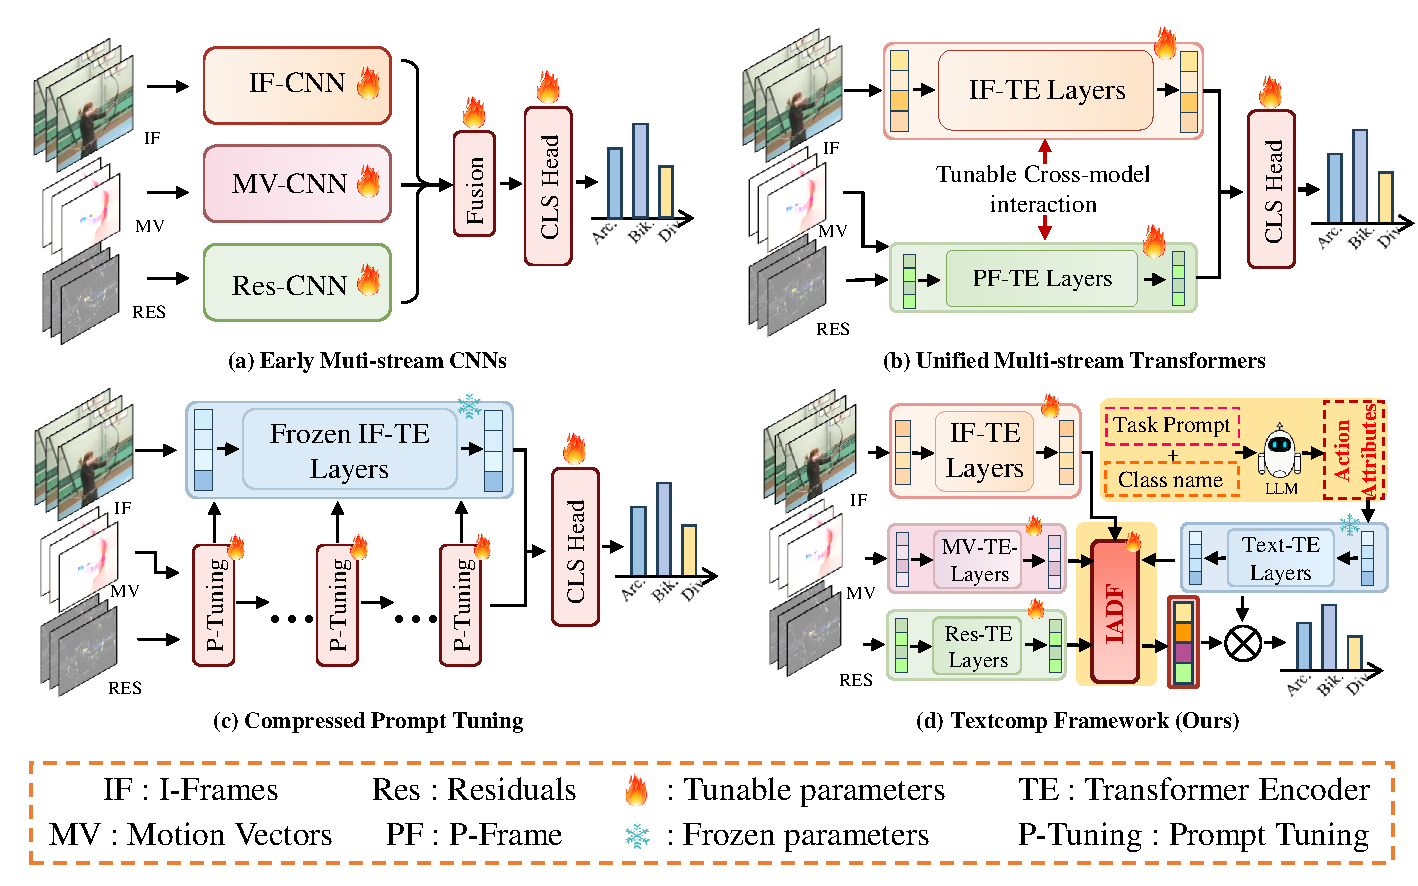
\includegraphics[width=\columnwidth]{figure/figure1-s.pdf}
\caption{Comparison of paradigms for compressed video action recognition. (a) Early multi-stream CNNs use separate branches for I-frames (IF), motion vectors (MV), and residuals (Res). (b) Unified multi-stream Transformers introduce visual cross-modal interaction between IF and P-frame encoders. (c) Compressed Prompt Tuning applies parameter-efficient visual adaptation to compressed videos. (d) TextComp uses LLM-generated action attributes as semantic anchors and IADF to adaptively route available codec evidence.}
\label{fig:type}
\end{figure}

Despite its efficiency, compressed-domain recognition faces a fundamental challenge: \emph{semantic sparsity}. An I-frame is a temporally sparse appearance observation, while MVs and residuals are codec-derived signals that are respectively coarse motion estimates and prediction errors. These heterogeneous streams retain useful evidence, but none alone provides a complete, high-level description of an action. As illustrated in Fig.~\ref{fig:type}, prior work primarily improves how these visual streams are encoded or fused: multi-branch CNNs process IF, MV, and Res separately \cite{battash2020mimic,huang2019flow,hu2023efficient,huo2021compressed,simonyan2014two}; unified multi-stream Transformers model visual interactions between IF and P-frame encoders \cite{chen2022mm,CFM-Net-li2025interactive,guo2026hierarchical}; and compressed prompt tuning adapts pre-trained visual models to codec signals \cite{li2023compressed}.

These approaches are complementary, but they operate within the compressed visual domain. They must decide which sparse, noisy cues are relevant to an action using the codec signals themselves. This differs from RGB-domain video recognition, where dense decoded frames expose richer appearance and temporal evidence. It also motivates a different role for language in the compressed domain: semantic priors can help navigate the available IF/MV/Res evidence, but cannot reconstruct fine-grained temporal interactions that are absent from the compressed representation.

Vision-language models (VLMs) show that language can provide high-level semantic cues for visual understanding. Existing RGB-domain VLM action-recognition methods use text together with decoded RGB video to improve visual-language alignment \cite{wang2021actionclipnewparadigmvideo,ni2022expanding}. In contrast, TextComp targets codec-domain streams and uses text to address their semantic sparsity. It is also distinct from visual-only compressed fusion methods, whose cross-modal interactions are driven only by IF/MV/Res features, and from compressed prompt tuning such as CVPT \cite{li2023compressed}, which generates visual prompts from compressed signals to adapt the visual encoder. Our goal is not to replace these visual representations or to claim complete fine-grained motion reasoning; it is to inject class-level semantic context into their use.

Accordingly, we propose TextComp (Fig.~\ref{fig:type}d), a text-guided semantic navigation framework for compressed video action recognition. An LLM decomposes each action label into multi-faceted attributes describing appearance, motion, and contextual cues. These attributes form a class-level semantic prior rather than a fixed assignment of semantics to IF, MV, or Res. The complete attribute sequence is available to every codec modality, allowing the model to determine its relevance from the visual evidence.

We instantiate this principle with an Instance-Aware Dynamic Fusion (IADF) module. IADF uses compressed visual features as queries to retrieve relevant attribute cues through cross-modal attention, then adaptively reweights codec features on an instance and frame basis. Thus, instance awareness arises from visual-query-based routing conditioned on class-level semantic priors, rather than from regenerating text for each video. The main contributions of this paper are:
\begin{itemize}
\item We formulate semantic sparsity as a central challenge in compressed video action recognition and introduce TextComp, which uses text-guided semantic navigation to enrich codec-domain representations.
\item We propose label-guided semantic attribute generation, which provides class-level appearance, motion, and contextual priors beyond coarse class names without enforcing a rigid semantic--modality decomposition.
\item We design an Instance-Aware Dynamic Fusion (IADF) module that uses visual-query-based cross-modal attention to adaptively route IF, MV, and Res features according to the available evidence in each video.
\item Experiments show that TextComp attains competitive compressed-domain performance with a favorable accuracy--efficiency trade-off and strong zero-/few-shot generalization, while fine-grained motion-centric recognition remains challenging for coarse codec signals.
\end{itemize}


\section{Related Work}
\label{sec:related_work}
\subsection{Action Recognition in Raw Videos}
Action recognition in the RGB domain exploits decoded frames and, in many cases, explicit motion representations. Two-Stream Networks \cite{simonyan2014two} combine RGB appearance with optical flow, while subsequent methods improve temporal modeling through segment-based, convolutional, or Transformer architectures \cite{wang2016temporal,xu2019dense,liu2022motion,piergiovanni2023rethinking}. More recent video VLMs align dense RGB video features with language to support recognition and transfer \cite{wang2021actionclipnewparadigmvideo,ni2022expanding}.

These RGB-domain approaches benefit from substantially richer visual evidence than codec-domain inputs: they can access decoded appearance at sampled frames and may compute or learn dense temporal features from it. In contrast, TextComp takes only IF, MV, and Res streams as visual inputs. It uses language not as a substitute for dense RGB evidence, but as a class-level prior that helps select and combine the limited semantic evidence retained by codec signals. This distinction makes raw-video VLM results useful references for the accuracy--efficiency trade-off, rather than directly equivalent comparisons.

\subsection{Action Recognition in Compressed Videos}
\label{subsec:compressed_learning}
\begin{figure*}[t!]
\centering
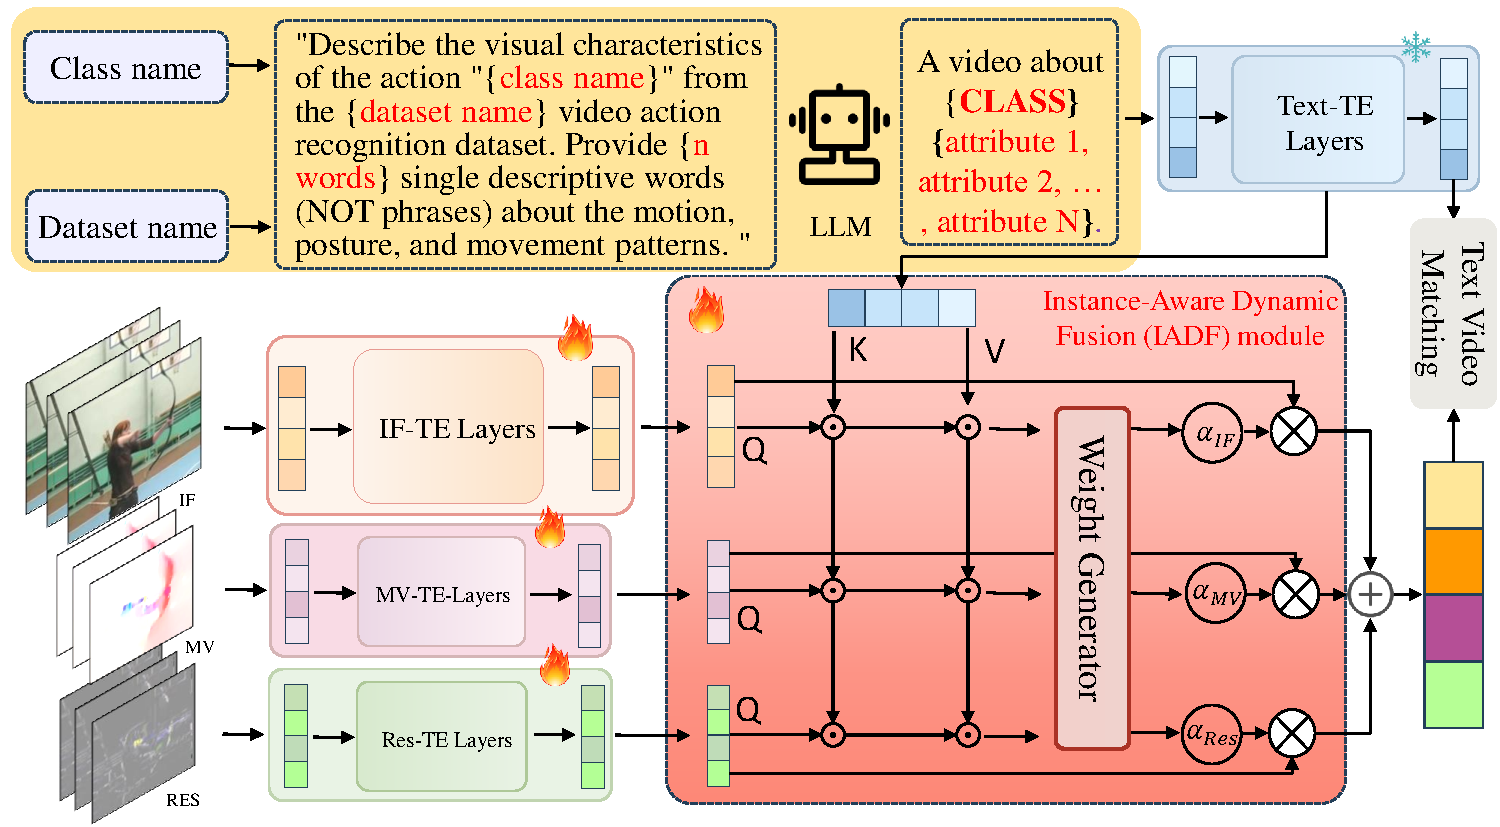
\includegraphics[width=\textwidth]{figure/figure2.pdf}
\caption{Overview of the \methodname framework. The visual branch encodes I-frames, motion vectors, and residuals into features. The textual branch produces class-level attribute embeddings. Visual-query-based cross-modal attention uses these embeddings to guide dynamic fusion for action classification.}
\label{fig:framework}
\end{figure*}
Early compressed-domain methods use MVs and residuals as efficient alternatives or complements to decoded RGB and optical flow \cite{zhang2016real,wu2018compressed}. Later work improves codec-domain representations by denoising MVs \cite{cao2019compressed}, generating flow-like motion cues \cite{shou2019dmc}, separating intra- and inter-frame dynamics \cite{li2020slow}, modeling visual modality interactions \cite{chen2022mm,CFM-Net-li2025interactive}, or exploiting GOP structure through self-supervision \cite{yu2020self}. These approaches demonstrate that IF, MV, and Res contain complementary visual evidence and motivate increasingly effective visual-only fusion.

TextComp is complementary to these methods rather than another visual fusion design. Visual-only fusion learns correlations among codec streams from the streams themselves; TextComp introduces class-level semantic attributes and uses visual-query-based attention to determine which available attribute cues are useful for each codec feature. This design targets the semantic sparsity of IF/MV/Res signals, while retaining the limitation that text guidance cannot restore fine-grained information absent from the codec representation.

\subsection{Parameter-Efficient Adaptation of Pre-trained Models}
\label{subsec:peft_adaptation}
The growth of large Vision Transformers (ViTs) and VLMs \cite{radford2021learning,yuan2021florence} has motivated parameter-efficient adaptation through prompts, adapters, and related lightweight modules. In computer vision, VPT \cite{jia2022visual} introduces learnable visual prompt tokens, while adapters and convolutional bypasses provide alternative efficient adaptation mechanisms \cite{chen2022adaptformer,jie2024convolutional}. Textual and multimodal prompting methods such as CoOp, Co-CoOp, MaPLe, and MMap adapt CLIP-style models by learning prompts in the text space, conditioning them on images, or coupling vision and language prompts \cite{zhou2022learning,zhou2022conditional,khattak2023maple,xin2024mmap}.

For compressed videos, CVPT \cite{li2023compressed} is particularly relevant because it generates \textit{visual prompts conditioned on compressed signals} such as MVs and residuals. CVPT therefore addresses how a pre-trained visual encoder can be adapted to the codec domain. TextComp addresses a different question: how class-level language semantics can navigate heterogeneous codec evidence after encoding. Our LLM-generated attributes are offline semantic priors, and IADF uses them for visual-query-based routing across IF, MV, and Res; it does not simply tune visual prompts or assume that a fixed semantic cue belongs to a particular modality. This distinction complements, rather than subsumes, parameter-efficient visual adaptation.

\section{Methodology}
\label{sec:method}

\subsection{Overview}
\label{sec:baseline}

Recent advances in vision-language models (VLMs), particularly CLIP~\cite{radford2021learning}, have demonstrated remarkable zero-shot and few-shot capabilities in raw video understanding~\cite{wang2021actionclipnewparadigmvideo,ni2022expanding}, leveraging natural language semantics to guide visual feature learning with superior generalization. However, existing compressed-domain methods~\cite{li2023compressed,CFM-Net-li2025interactive} rely solely on visual encoders without textual supervision, limiting their ability to capture high-level semantics. To bridge this gap, we introduce TextComp, the first CLIP-based framework for compressed-domain action recognition, enabling semantic-aware multimodal fusion through vision-language alignment.

As illustrated in Fig.~\ref{fig:framework}, our framework processes visual and textual information in dual parallel branches. For the visual branch, we extract three compressed-domain modalities from the video bitstream: sparse I-frames $\mathbf{F}_{IF}$, motion vectors $\mathbf{F}_{MV}$, and residuals $\mathbf{F}_{Res}$. I-frames are encoded by the pre-trained CLIP visual encoder to obtain $\mathbf{V}_{IF}$, while motion vectors and residuals use lightweight 2-layer encoders initialized from the first and last layers of the CLIP visual encoder, producing $\mathbf{V}_{MV}, \mathbf{V}_{Res}$. This transfers CLIP's visual priors to codec-specific modalities while maintaining efficiency.

For the textual branch, we leverage fine-grained attribute descriptions beyond simple class names to provide richer semantic supervision (Sec.~\ref{sec:attribute}). These attribute-enhanced representations serve as semantic anchors, guiding our Instance-Aware Dynamic Fusion (IADF) module to selectively aggregate compressed-domain features based on action-specific semantic requirements (Sec.~\ref{sec:fusion}).

\subsection{Label-Guided Semantic Attribute Generation}
\label{sec:attribute}

\noindent\textbf{Attribute Generation.} 
Existing vision-language methods for action recognition~\cite{wang2021actionclipnewparadigmvideo,ni2022expanding} typically rely on class names or learnable prompt tokens~\cite{zhou2022learning} for textual supervision, which provide only coarse-grained categorical information. Moreover, video action categories inherently exhibit low semantic distinction, making it challenging to differentiate similar actions based solely on class names. When introducing compressed-domain modalities into CLIP-based frameworks, this limitation becomes more pronounced: I-frames capture appearance and object information, motion vectors encode movement patterns, and residuals represent temporal changes---each modality conveys distinct semantic aspects that cannot be adequately described by simple class names alone. To address this, we enrich the textual context with attributes---words highly correlated with each action class---that provide fine-grained semantic cues explicitly associated with different compressed-domain modalities, thereby fully leveraging the capabilities of vision-language models.

Specifically, we leverage large language models (Llama 3.1-8B) to generate $L=32$ descriptive attribute words for each action category. This generation is performed offline once for the category vocabulary and introduces no LLM overhead during inference. We design a prompt template that instructs the model to output single words describing the motion patterns, involved objects, body postures, and movement characteristics:
\begin{quote}
\textit{Describe the visual characteristics of the action ``\{class\_name\}'' from the \{dataset\_name\} video action recognition dataset. Provide \{n\_words\} single descriptive words (NOT phrases) about the motion, posture, and movement patterns.}
\end{quote}
After quality filtering (removing symbols, non-alphabetic words, and duplicates), the cleaned attribute set $\mathcal{A}_c = \{a_1^c, ..., a_L^c\}$ is structured into a prompt template: ``\textit{a video about \{class\_name\} \{attribute\_1\} \{attribute\_2\} ... \{attribute\_L\}}''. These constructed prompts are then converted into a sequence of embeddings $\mathbf{T}_A \in \mathbb{R}^{L \times D}$ via the CLIP text encoder, serving as the multi-faceted textual supervision for our model.

\noindent\textbf{Implicit Semantic Routing.} 
Instead of projecting these attributes into predefined, static semantic sub-spaces, we allow the network to implicitly determine the semantic relevance of each modality dynamically. Different actions exhibit varying degrees of dependence on compressed-domain modalities (e.g., ``running'' relies heavily on motion vectors while ``reading'' depends primarily on I-frame appearance). We feed the entire sequence of attribute embeddings $\mathbf{T}_A$ directly into our fusion module, utilizing cross-modal attention to let the visual modalities adaptively "query" the exact semantic cues they require.

\subsection{Instance-Aware Dynamic Fusion (IADF)}
\label{sec:fusion}

To effectively leverage the generated semantic cues to guide the fusion of heterogeneous compressed-domain features, we propose the Instance-Aware Dynamic Fusion (IADF) module. This module dynamically modulates the integration of I-frames, motion vectors, and residuals based on fine-grained, frame-level semantic intent, while employing feature-level semantic injection and learnable gating strategies to optimize the pre-trained representation space smoothly.

\noindent\textbf{Cross-Modal Semantic Injection.} 
We first employ a cross-modal attention mechanism to evaluate the relevance of each visual modality to the provided semantic attributes. The visual features of each modality $\mathbf{V}_i$ for $i \in \{\text{IF}, \text{MV}, \text{Res}\}$ act as queries, while the attribute sequence $\mathbf{T}_A$ serves as keys and values. To preserve the linguistic semantic space while allowing the fusion module to provide informative gradient feedback to the visual backbones, we apply a stop-gradient operation, denoted as $\text{sg}(\cdot)$, exclusively to the text attributes:
$$\mathbf{Q}_i = \mathbf{V}_i\mathbf{W}_{Q,i}, \quad \mathbf{K} = \text{sg}(\mathbf{T}_A)\mathbf{W}_K, \quad \mathbf{V} = \text{sg}(\mathbf{T}_A)\mathbf{W}_V$$
$$\mathbf{Z}_i = \text{softmax}\left(\frac{\mathbf{Q}_i \mathbf{K}^\top}{\sqrt{d}}\right)\mathbf{V}$$
where $\mathbf{Z}_i$ represents the semantic-injected features for modality $i$ at the frame level. Instead of directly fusing the original visual modalities, we explicitly inject these instance-aware semantic features back into the visual space via a residual connection. Using a projection matrix $\mathbf{W}_{P,i}$ and a modality-specific learnable scale parameter $\gamma_i$, we obtain the enhanced visual representations:
$$\hat{\mathbf{V}}_i = \mathbf{V}_i + \gamma_i (\mathbf{Z}_i \mathbf{W}_{P,i})$$
This semantic injection ensures that even prior to weight-based routing, the visual features themselves inherently possess instance-aware attributes.

\noindent\textbf{Dynamic Frame-Level Routing.} 
To compute fine-grained, frame-specific fusion weights, we utilize the temporal dimension of our features. We concatenate the frame-level semantic-injected features $\mathbf{Z}_i$ alongside a globally pooled attribute representation $\mathbf{t}_{global} = \text{MeanPool}(\text{sg}(\mathbf{T}_A))$ (expanded along the temporal dimension) to form a comprehensive routing state at each time step $t$: $\mathbf{r}_t = [\mathbf{Z}_{\text{IF}, t} \parallel \mathbf{Z}_{\text{MV}, t} \parallel \mathbf{Z}_{\text{Res}, t} \parallel \mathbf{t}_{global}]$. We map this state to weight residuals via a Multilayer Perceptron (MLP) equipped with Layer Normalization to stabilize feature variance:
$$\Delta \mathbf{w}_t = g \cdot \mathbf{W}_{out} (\text{LayerNorm}(\text{GELU}(\mathbf{W}_{in}\mathbf{r}_t)))$$
To ensure smooth optimization and prevent premature disruption of the base fusion distribution, we introduce a learnable gating parameter $g$, initialized to a small scalar (e.g., $0.01$). This soft-gating mechanism replaces rigid clamping or zero-initialization, preserving the natural weight initialization distribution while ensuring the dynamic router initially outputs near-zero residuals ($\Delta \mathbf{w}_t \approx \mathbf{0}$).



\begin{table*}[ht]  
    \centering
    \scriptsize
    \caption{Performance comparison with representative raw-video and compressed-domain methods on Kinetics-400. Raw-video methods are included as efficiency references, while compressed-domain methods are the primary comparison group.}
    % 使用 resizebox 强制表格适应文本宽度，解决与右侧行号重叠的问题
    \resizebox{\textwidth}{!}{%
    \begin{tabular}{c|c|c|c|c|c|c|c}
        \hline
            \multicolumn{2}{c|}{Method}& Modality & Backbone & GFLOPs & Top-1 & Top-5 & Zero-shot\\
        \hline
        \multirow{8}{*}{\rotatebox{90}{\bf{Raw}}} 
        & MVFNet  \cite{mvfnet}& RGB & ResNet50 & 1974.0 & 77.0 & 92.8 & \ding{56} \\
        & TEA \cite{li2020tea} &  RGB &  ResNet50 & 2100.0 & 75.0 & 92.8 & \ding{56} \\ 
        & TDN \cite{wang2021tdn} &  RGB&  ResNet50 & 3240.0 & 76.6 & 92.8 & \ding{56} \\ 
        & VideoMAE  \cite{videomae} & RGB & ViT-B & 1080.0 & 81.5 & 95.1 & \ding{56} \\
        & ActionCLIP  \cite{wang2021actionclipnewparadigmvideo} & RGB+Text & ViT-B & 563 & 83.8 & 96.2 & \ding{52}\\
        & M$^{2}$-CLIP \cite{wang2024m2} & RGB+T & ViT-B & 422 & 83.4 & 96.7 & \ding{52}\\
        & Vita-CLIP  \cite{wasim2023vitaclipvideotextadaptive} & RGB+Text & ViT-B & 190 & 82.9 & 96.3 & \ding{52}\\
        & X-CLIP \cite{ni2022expanding} & RGB+T & ViT-B & 145 & 83.8 & 96.7 & \ding{52}\\
        \hline 
        \hline 
        \multirow{5}{*}{\rotatebox{90}{\bf{Comp.}}}
        & MFCD-Net \cite{battash2020mimic} & I+M+R & MFNet3D & 1300.0 & 68.3 & - & \ding{56} \\
        & MEACI-Net \cite{li2022representation}& I+M+R & I3D & 269.4 & 71.5 & - & \ding{56}\\
        % 修复了此处原代码中结尾的 \\\ 语法错误
        & DSDMT$^{R*}$~\cite{DSDMT} & I+M+R & ResNet101 & 141 & 74.1 & - & \ding{56}\\
        & CoViFocus~\cite{zheng2023dynamic} & I+M & ResNet50 & 296 & 72.0 & - & \ding{56}\\
        \cline{2-8}
        & \textbf{\methodname~(Ours)}  & I+M+R+Text & ViT/B & 145.8 & \textbf{80.3} & \textbf{94.5} & \ding{52}\\
        \hline
    \end{tabular}%
    }

    \label{tab:kinetics400}
\end{table*}

\noindent\textbf{Adaptive Fusion.} 
The generated frame-level dynamic residuals $\Delta \mathbf{w}_t \in \mathbb{R}^3$ are added to a set of learnable base weights $\boldsymbol{\beta} \in \mathbb{R}^3$, which capture the dataset-level global modality preferences. The final fusion weights for each frame are normalized via a softmax function:
$$\boldsymbol{\alpha}_t = \text{softmax}(\boldsymbol{\beta} + \Delta \mathbf{w}_t)$$



Finally, the semantic-enhanced visual modalities $\hat{\mathbf{V}}_i$ are aggregated along the temporal dimension using these dynamically generated, frame-specific weights:
$$\mathbf{V}_{\text{fused}, t} = \sum_{i \in \{\text{IF}, \text{MV}, \text{Res}\}} \alpha_{i, t} \hat{\mathbf{V}}_{i, t}$$
This formulation ensures that the primary visual backbones receive active gradient guidance to extract fusion-friendly representations, while the cross-modal semantic guidance dynamically adapts to both the instance-level and frame-level requirements of each video.

%-------------------------------------------------------------------------


\section{Experimental Results and Analysis}
\label{sec:experiments} % Add label for cross-referencing

\begin{table*}[ht]  
    \centering
    \caption{Performance comparison with representative raw-video and compressed-domain methods on HMDB-51, UCF-101, and Something-Something v2 (SSv2). Raw-video methods are included as efficiency references, while compressed-domain methods are the primary comparison group.}
    \resizebox{\textwidth}{!}{%
    \begin{tabular}{c|c|c|c|c|c|c|c|c}
        \hline
         \multicolumn{2}{c|}{Method} & Modality & Backbone & GFLOPs  & HMDB-51 & UCF-101 & SSv2 & Zero-shot\\
        \hline
        \multirow{6}{*}{\rotatebox{90}{\bf{Raw}}}
        & MVFNet  \cite{mvfnet}& RGB & ResNet50 & 1974.0 & 75.7 & 96.6 & 63.5 &  \ding{56} \\
        & TEA \cite{li2020tea} &  RGB &  ResNet50 & 2100.0 & 73.3 & 96.9 & 48.9 &  \ding{56} \\ 
        & TDN \cite{wang2021tdn} &  RGB&  ResNet50 & 3240.0 & \textbf{76.3} & \textbf{97.4} & 65.3 & \ding{56}\\ 
        & VideoMAE  \cite{videomae} & RGB & ViT-B & 1080.0 & 73.3 & 96.1 & \textbf{69.9} & \ding{56}\\
        & Vita-CLIP  \cite{wasim2023vitaclipvideotextadaptive} & RGB+T & ViT-B & 190 & - & - & 48.7 & \ding{52}\\
        & M$^{2}$-CLIP \cite{wang2024m2} & RGB+T & ViT-B & 422 & - & - & 66.9 & \ding{52}\\
        \hline 
        \hline 
        \multirow{16}{*}{\rotatebox{90}{\bf{Comp.}}}
        & IPTSN  \cite{huang2019flow} & I+M+R & ResNet152 & 215.0 & 69.1 & 93.4 & - & \ding{56}\\
        & CoViAR  \cite{wu2018compressed} & I+M+R & ResNet152 & 1222.0 & 59.1 & 90.4 & - &  \ding{56}\\
        & CoViAR  \cite{wu2018compressed} & I+M+R+F & ResNet152 & 3970.0& 70.2 & 94.9 & -&  \ding{56}\\
        & DMC-Net  \cite{shou2019dmc} & I+M+R+F & I3D & 401.0& 71.8 & 92.3 & - &  \ding{56}\\
        & SIFT-Net  \cite{li2020slow} & I+M+R & I3D & 1971.0 & 72.3 & 94.0 & - &  \ding{56}\\
        & MFCD-Net \cite{battash2020mimic} & I+M+R & MFNet3D & 1300.0 & 66.9 & 93.2 & - & \ding{56}\\
        & MEACI-Net \cite{li2022representation}& I+M+R & I3D & 269.4 & 74.4 & 96.4 & - & \ding{56}\\
        & DSDMT$^{R*}$~\cite{DSDMT} & I+M+R & ResNet101 & 141 & 74.9 & 95.8 & -& \ding{56}\\
        & CoViFocus~\cite{zheng2023dynamic} & I+M & ResNet50 & 296 & 74.8 & 95.8 & - & \ding{56}\\
        & MussNet~\cite{MussNetterao2024multi} & I+M+R & ResNet50-TSM & 38.7 & 63.7 & 89.1 & - & \ding{56} \\
        & MussNet-LF~\cite{LF-terao2023efficient} & I+M+R & ResNet50 & 33.6 & 62.9 & 89.2 & -  & \ding{56}\\
        & PKD+WISE~\cite{PKD-WISE-soufleri2024advancing} & I+M+R & ResNet152 & - & 68.2 & 92.9 & - & \ding{56}\\
        & CFM-Net~\cite{CFM-Net-li2025interactive} & I+M+R & UniFormer & 48 & 75.7 & 94.8 & -  & \ding{56}\\
        & MM-ViT  \cite{chen2022mm}& I+M+R & ViT/B & 820 & - & 93.3 & \textbf{64.9} & \ding{56}\\
        & CVPT  \cite{li2023compressed}& I+M+R & ViT/B & 772.2 & 69.7 & 95.5 & -  & \ding{56}\\
        \cline{2-9} 
        & \methodname~(Ours)  & I+M+R+T & ViT/B & 145.8 & \textbf{76.2} & \textbf{96.7} & 60.4 & \ding{52}\\
        \hline
    \end{tabular}%
    }
    \label{tab:ssv2}
\end{table*}


% 表1：Zero-shot
\begin{table*}[tb]
\centering
\caption{Comparison for zero-shot performances on HMDB51 and UCF101.}
\label{tab:zeroshothmdbucf}
\begin{tabular}{lccc}
\toprule
Method & Modality & HMDB-51 & UCF-101 \\
\midrule
ActionCLIP~\cite{wang2021actionclipnewparadigmvideo} & RGB+T & 40.8 \ensuremath{\pm} 5.4 & 58.3 \ensuremath{\pm} 3.4 \\
X-CLIP~\cite{ni2022expanding} & RGB+T & 44.6 \ensuremath{\pm} 5.2 & 72.0 \ensuremath{\pm} 2.3 \\
Vita-CLIP~\cite{wasim2023vitaclipvideotextadaptive} & RGB+T & 48.6 \ensuremath{\pm} 0.6 & 75.0 \ensuremath{\pm} 0.6 \\
M$^{2}$-CLIP~\cite{wang2024m2} & RGB+T & 47.1 \ensuremath{\pm} 0.4 & 78.7 \ensuremath{\pm} 1.2 \\
ViFi-CLIP~\cite{rasheed2023fine} & RGB+T & \textbf{51.3 \ensuremath{\pm} 0.6} &\textbf{ 76.8 \ensuremath{\pm} 0.}7 \\
\midrule
\methodname~(Ours) & I+M+R+T & \textbf{49.4 \ensuremath{\pm} 1.1} & \textbf{73.6 \ensuremath{\pm} 1.0} \\
\bottomrule
\end{tabular}
\end{table*}

% 表2：Few-shot (保留了 resizebox 以防超宽，并使用 cmidrule 分割子表头)
\begin{table*}[tb]
\centering
\caption{Comparison for few-shot performances on HMDB51 and UCF101.}
\label{tab:fewshothmdb}
% \resizebox{\textwidth}{!}{%
\begin{tabular}{lccccccccc}
\toprule
\multirow{2}{*}{Method} & \multirow{2}{*}{Modality} & \multicolumn{4}{c}{HMDB-51} & \multicolumn{4}{c}{UCF-101} \\
\cmidrule(lr){3-6} \cmidrule(lr){7-10}
& & K=2 & K=4 & K=8 & K=16 & K=2 & K=4 & K=8 & K=16 \\
\midrule
ActionCLIP~\cite{wang2021actionclipnewparadigmvideo} & RGB+T & 55.0 & 56.0 & 58.0 & - & 80.0 & 85.0 & 89.0 & - \\
X-CLIP~\cite{ni2022expanding} & RGB+T & 53.0 & 57.3 & 62.8 & 64.0 & 76.4 & 83.4 & 88.3 & 91.4 \\
X-Florence~\cite{ni2022expanding} & RGB+T & 51.6 & 57.8 & 64.1 & 64.2 & \textbf{84.0} & \textbf{88.5} & \textbf{92.5} & \textbf{94.8} \\
ViFi-CLIP~\cite{rasheed2023fine} & RGB+T & \textbf{57.2} & \textbf{62.7} & \textbf{64.5} & \textbf{66.8} & 80.7 & 85.1 & 90.0 & 92.7 \\
\midrule
\methodname~(Ours) & I+M+R+T & \textbf{65.2} & \textbf{65.3} & \textbf{67.2} & \textbf{70.9} & \textbf{91.1} & \textbf{92.9} & \textbf{94.6} & \textbf{95.4} \\
\bottomrule
\end{tabular}%
% }
\end{table*}


\subsection{Dataset}
We evaluate our model on four widely used video action recognition benchmarks of varying scale and complexity: UCF-101, HMDB-51, Something-Something v2 (SSv2), and Kinetics-400. UCF-101 and HMDB-51 are relatively small datasets, containing 13,320 videos across 101 classes and 6,766 videos across 51 classes, respectively. In contrast, SSv2 and Kinetics-400 are large-scale benchmarks; SSv2 focuses on fine-grained motion reasoning with 168,913 training and 24,777 validation videos spanning 174 categories, while Kinetics-400 includes approximately 240K training and 20K validation clips across 400 diverse human actions.

We use top-1 accuracy as the evaluation metric. For UCF-101 and HMDB-51, we follow the standard evaluation protocol and report the mean performance across the three official splits~\cite{wu2018compressed,li2023compressed}.

\subsection{Implementation Details}

Following \cite{wu2018compressed}, we used MPEG-4 encoded videos with an average of 11 P-frames per I-frame, uniformly resizing video resolution to $340 \times 256$. Sixteen clips were uniformly sampled from each video, with their spatiotemporal positions determined by the GOP structure: random GOP indices and intra-clip position sampling were employed during training for data augmentation, while deterministic center sampling was applied during testing. Spatial processing included random corner cropping and horizontal flipping during training, and center cropping during testing, with consistent spatial dimension handling across all inputs. For the backbone network, we adopt CLIP ViT-B/16 as the encoder for I-frame streams. The text encoder from CLIP ViT-B/32 is employed to encode textual information. The base learning rate, weight decay, and batch size are set to $5\times 10^{-5}$, $2\times 10^{-2}$, and 32, respectively. The model is trained for 20 epochs with a learning rate warm-up strategy applied during the first 5 epochs. All experiments are conducted on two NVIDIA 4090D GPUs.



\subsection{Fully-Supervised Experiments}
Table~\ref{tab:kinetics400} presents the results on Kinetics-400. \methodname~achieves \textbf{80.3\%} top-1 accuracy, surpassing previous compressed-domain methods by significant margins: \textbf{+6.2\%} over DSDMT~\cite{DSDMT} and \textbf{+8.8\%} over MEACI-Net~\cite{li2022representation}, while requiring only 145.8 GFLOPs. While \methodname's accuracy is slightly lower than some raw-video VLM-based approaches (e.g., ActionCLIP: 83.8\%), this gap is primarily due to the inherent information loss in compressed representations—sparse I-frames and coarse motion vectors cannot fully capture dense temporal dynamics. Nevertheless, \methodname~achieves highly competitive performance with dramatically reduced computational cost (76\% fewer GFLOPs than ActionCLIP), proving the efficacy of introducing vision-language alignment into the compressed domain.

Table~\ref{tab:ssv2} shows the results on HMDB-51, UCF-101, and SSv2. On HMDB-51, \methodname~achieves \textbf{76.2\%}, outperforming DSDMT (74.9\%) and CoViFocus (74.8\%). On UCF-101, we obtain \textbf{96.7\%}, surpassing DSDMT (95.8\%). For the motion-centric SSv2 dataset, \methodname~achieves \textbf{60.4\%}. The larger gap compared to raw-video methods (e.g., VideoMAE: 69.9\%) is expected, as SSv2 emphasizes fine-grained temporal reasoning that is particularly challenging for compressed representations. Overall, \methodname~achieves a favorable accuracy-efficiency trade-off among compressed-domain approaches, while its remaining gap on SSv2 highlights the intrinsic difficulty of fine-grained motion reasoning from coarse motion vectors.

\subsection{Zero-Shot Experiments}
\noindent\textbf{Settings.} We evaluate zero-shot generalization on HMDB-51 and UCF-101 using models pre-trained on Kinetics-400, strictly following X-CLIP~\cite{ni2022expanding} protocols. Results are reported as "average \ensuremath{\pm} standard deviation" across three splits.

\noindent\textbf{Results.} As shown in Table~\ref{tab:zeroshothmdbucf}, \methodname~achieves \textbf{49.4\ensuremath{\pm}1.1\%} on HMDB-51 and \textbf{73.6\ensuremath{\pm}1.0\%} on UCF-101. While lower than some raw-video methods (e.g., ViFi-CLIP), \methodname~demonstrates robust zero-shot capabilities despite the limitations of compressed-domain modalities. Notably, we outperform M\ensuremath{^2}-CLIP (47.1\%) on HMDB-51 and surpass ActionCLIP (58.3\%) and X-CLIP (72.0\%) on UCF-101 by substantial margins. This competitive performance validates that our label-guided semantic attribute generation provides rich textual anchors, enabling effective generalization to unseen categories even without dense visual information.

\subsection{Few-Shot Comparisons}
\noindent\textbf{Settings.} We evaluate few-shot learning on HMDB-51 and UCF-101 by randomly sampling K={2, 4, 8, 16} videos per class from Kinetics-400 pre-trained models.

\noindent\textbf{Results.} Table~\ref{tab:fewshothmdb} demonstrates \methodname's remarkable few-shot performance. In the 2-shot scenario on HMDB-51, \methodname~achieves \textbf{65.2\%}, surpassing ViFi-CLIP by \textbf{8.0\%}. This advantage persists across all settings: \textbf{+2.6\%} at K=4, \textbf{+2.7\%} at K=8, and \textbf{+4.1\%} at K=16. Similar improvements are consistently observed on UCF-101. The superior few-shot performance highlights the effectiveness of our attribute-guided semantic decomposition, which explicitly models correspondences between action attributes and compressed modalities, allowing the model to quickly adapt to novel categories using minimal samples.


\subsection{Ablation Study}
We select the most diagnostic ablations on HMDB-51 and UCF-101 to isolate the source of improvement, rather than only reporting isolated component gains. These results answer three questions: whether compressed modalities beyond I-frames are necessary, whether gains come from meaningful semantics rather than longer prompts, and whether IADF contributes beyond static fusion.

\begin{table*}[tb]
\centering
\caption{Ablations that disentangle the sources of improvement. ``Semantic Match'' indicates whether the textual attributes correspond to the correct action category.}
\label{tab:source_ablation}
\begin{tabular}{llccc}
\toprule
Setting & Text Supervision & Semantic Match & HMDB-51 & UCF-101 \\
\midrule
IF only & w/o attributes & -- & 74.2 & 95.5 \\
IF only & w/ attributes & \ding{52} & 73.4 & 95.4 \\
I+MV+Res & Class name only & \ding{52} & 74.4 & 95.1 \\
I+MV+Res & Dummy prompt & \ding{56} & 74.2 & 95.3 \\
I+MV+Res & Shuffled attributes & \ding{56} & 74.2 & 95.5 \\
I+MV+Res & Correct attributes & \ding{52} & 75.9 & 96.4 \\
I+MV+Res+IADF & Correct attributes & \ding{52} & \textbf{76.2} & \textbf{96.7} \\
\bottomrule
\end{tabular}
\end{table*}

\noindent\textbf{Source of Improvement.} Table~\ref{tab:source_ablation} shows that I-frames alone are insufficient for compressed-domain recognition: adding MV/Res cues and semantic attributes improves the model from 74.2/95.5 to 75.9/96.4. More importantly, the improvement is not caused by prompt length or additional tokens. A category-agnostic dummy prompt and shuffled attributes do not improve over the class-name baseline, while correct attributes consistently help. This confirms that the benefit comes from meaningful semantic matching between action attributes and compressed visual signals.

\begin{table}[tb]
\centering
\caption{Ablative evaluation of fusion strategies.}
\label{tab:FusionWeight}
\begin{tabular}{lcc}
\toprule
Fusion Strategy & HMDB-51 & UCF-101 \\
\midrule
Fixed weights & 75.9 & 96.4 \\
Trainable weights & 76.0 & 96.5 \\
IADF (Ours) & \textbf{76.2} & \textbf{96.7} \\
\bottomrule
\end{tabular}
\end{table}

\noindent\textbf{Effectiveness of IADF.} Table~\ref{tab:FusionWeight} compares fixed fusion, naive trainable fusion, and the proposed IADF. IADF performs best on both datasets, indicating that instance-aware semantic routing provides additional gains beyond simply learning global modality weights.

\begin{table}[tb]
\centering
\caption{Robustness of attribute generation and prompt design on HMDB-51.}
\label{tab:attribute_robustness}
\begin{tabular}{lcc}
\toprule
Evaluation & Protocol & Top-1 \\
\midrule
LLM generator & Qwen3:8B & 76.0 \\
LLM generator & Llama3.1:8B & \textbf{76.2} \\
Generation variance & 5 regenerations & 75.8$\pm$0.3 \\
Prompt sensitivity & 5 templates & 76.0$\pm$0.4 \\
Attribute source & Manual & 74.1 \\
Attribute source & LLM & 75.6 \\
Attribute source & LLM + manual selection & \textbf{77.8} \\
\bottomrule
\end{tabular}
\end{table}

\noindent\textbf{Attribute Robustness.} Table~\ref{tab:attribute_robustness} summarizes the robustness of the textual branch. Different LLM generators produce similar performance, and repeated generation or prompt-template changes lead to small variance. The comparison between manual and LLM-generated attributes further suggests that LLM attributes provide a strong and convenient semantic prior, while manual selection can serve as an upper-bound quality check.

\begin{table}[tb]
\centering
\caption{Semantic separability of text features on HMDB-51. Lower values indicate better inter-class discriminability.}
\label{tab:semantic_sim_main}
\begin{tabular}{lcc}
\toprule
Prompt Strategy & Off-diag. Sim. $\downarrow$ & Top-1 Conf. $\downarrow$ \\
\midrule
Class name only & 0.8418 & 0.9087 \\
w/o Dataset Name & 0.8018 & 0.8926 \\
w/ Dataset Name & \textbf{0.7593} & \textbf{0.8604} \\
\bottomrule
\end{tabular}
\end{table}

\noindent\textbf{Semantic Discriminability.} Table~\ref{tab:semantic_sim_main} analyzes CLIP text features before visual training. Attribute-enhanced prompts reduce inter-class similarity compared with class names alone, and dataset-aware attributes yield the most discriminative textual space. This explains why attribute prompts are more effective than coarse class-name supervision for visually similar action categories.

\begin{figure}[tb]
\centering
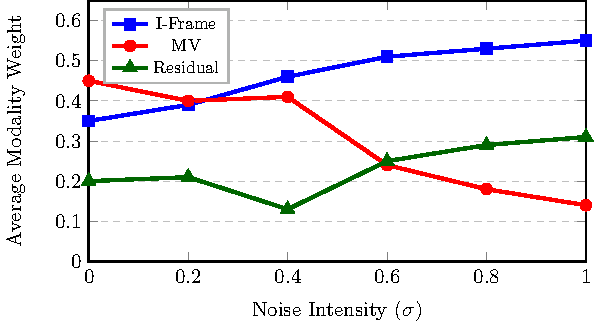
\includegraphics[width=0.8\linewidth]{figure/figure3.pdf}
\caption{Modality weight adaptation under MV noise injection.}
\label{fig:noise_injection}
\end{figure}

\noindent\textbf{Routing Behavior and Robustness.} To simulate unreliable codec signals, we inject Gaussian noise $\mathcal{N}(0, \sigma^2)$ into MV features during inference. As shown in Fig.~\ref{fig:noise_injection}, IADF decreases the corrupted MV weight and increases reliance on I-frame and residual features as noise grows. Class-level routing statistics also show that IADF does not collapse to a single modality: on HMDB-51, I-frame, MV, and residuals dominate 22, 10, and 19 classes respectively. Motion-centric actions such as throw, handstand, turn, and cartwheel assign higher weights to MV+Res, whereas appearance- or object-related actions such as shoot gun, sword, sit, and smoke rely more on I-frames.

\noindent\textbf{Discussion on SSv2.} SSv2 emphasizes fine-grained temporal transformations, which are difficult to recover from coarse motion vectors. Our lower absolute SSv2 accuracy should therefore be interpreted as a limitation of compressed representations rather than a failure of semantic routing. In fact, IADF improves SSv2 from 57.7\% to 60.4\% by increasing the contribution of motion-related MV/Res branches compared with trainable fusion.

\begin{table}[tb]
\centering
\caption{Comparison of inference time (ms) per video.}
\label{tab:inferenceefficiency}
\begin{tabular}{lccc}
\toprule
Method & \shortstack{Pre-\\process} & Inference & \shortstack{Full\\Pipeline} \\
\midrule
ActionCLIP~\cite{wang2021actionclipnewparadigmvideo} & 41.51 & \textbf{11.52} & 53.03 \\
\methodname~(Ours) & \textbf{6.11} & 14.23 & \textbf{20.34} \\
\bottomrule
\end{tabular}
\end{table}

\noindent\textbf{Inference Efficiency.} Attribute generation is performed offline, and the deployed model only consumes compressed-domain streams and stored text embeddings. As shown in Table~\ref{tab:inferenceefficiency}, avoiding full RGB decoding reduces preprocessing time from 41.51 ms to 6.11 ms and yields a 2.6$\times$ faster full pipeline than ActionCLIP.

\section{Conclusions}
\label{sec:conclusion}
In this paper, we proposed TextComp, a novel framework that bridges the semantic gap in compressed video action recognition via text-guided navigation. By leveraging Large Language Models (LLMs) to decompose action categories into multifaceted semantic attributes. To fully exploit these textual priors without collapsing pre-trained feature spaces, we designed the Instance-Aware Dynamic Fusion (IADF) module, which adaptively routes visual features based on semantic queries. Extensive experiments across four benchmarks demonstrate that TextComp effectively balances computational efficiency, recognition accuracy, and zero-/few-shot generalization in compressed-domain video understanding. These results validate the immense potential of vision-language synergy in resource-constrained video understanding.
\bibliography{aaai2027}

% Check whether the conference requires a reproducibility checklist to be included in the paper.
% If so, you can uncomment the following line and ajust the path to include it.
% \input{ReproducibilityChecklist.tex}

\end{document}
